\chapter{Introduction} \label{chap:intro}
A gentle reminder not to get this chapter perfect until the dissertation is nearing its completion\ldots

\section{A section}

\subsection{A sub-section}

\subsubsection{A sub-sub-section}



\section{Citations}



\section{Figures}

\begin{figure}
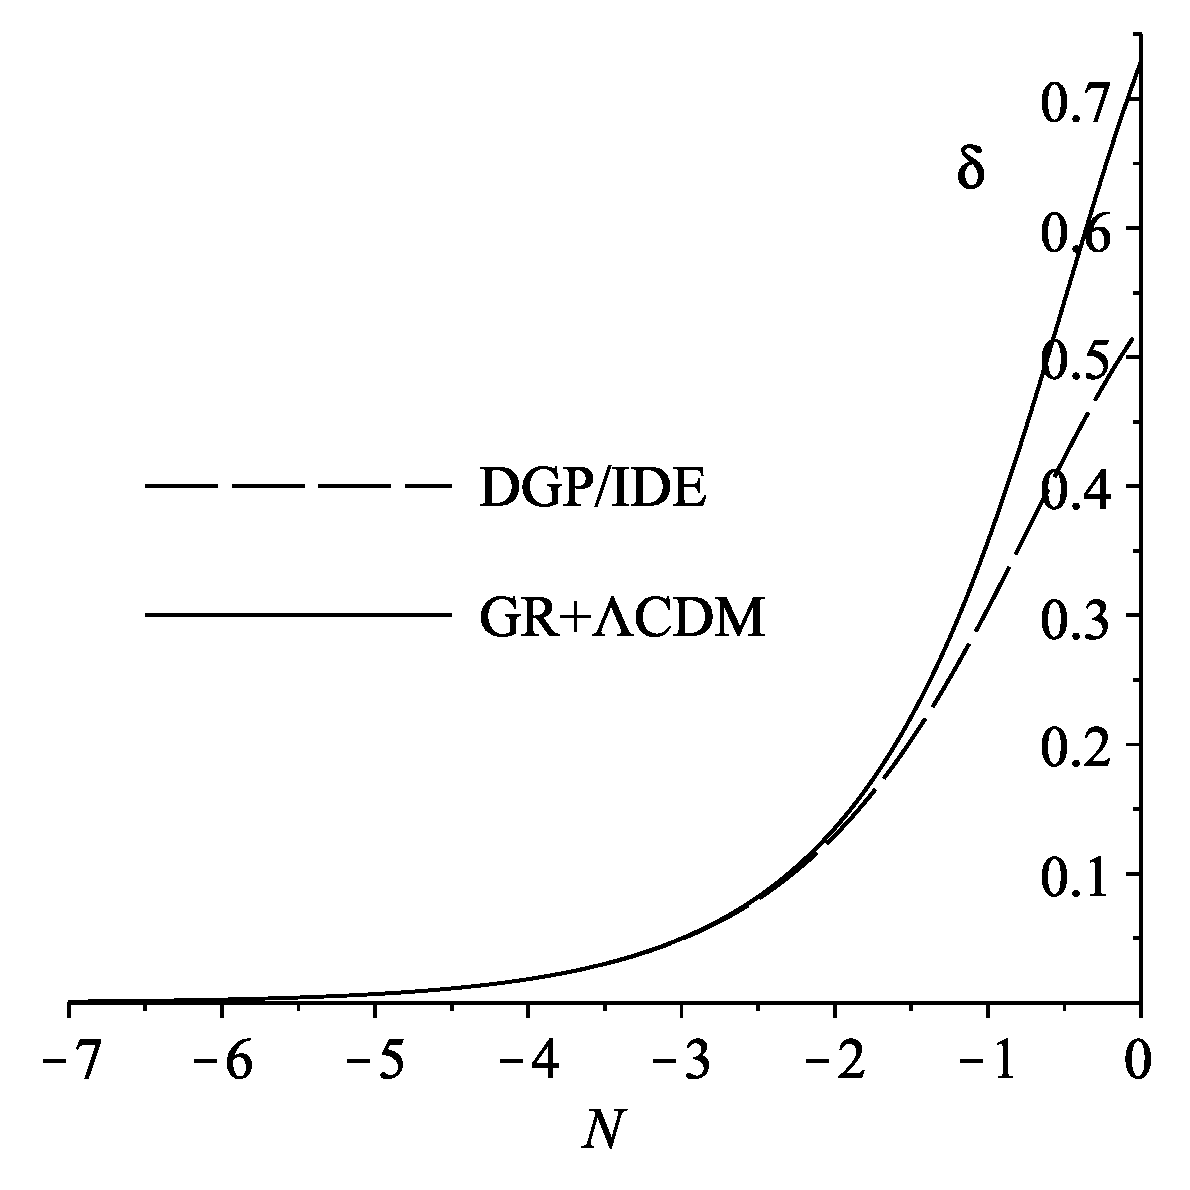
\includegraphics[width=0.49\columnwidth]{figures/dgpdeltas.eps}
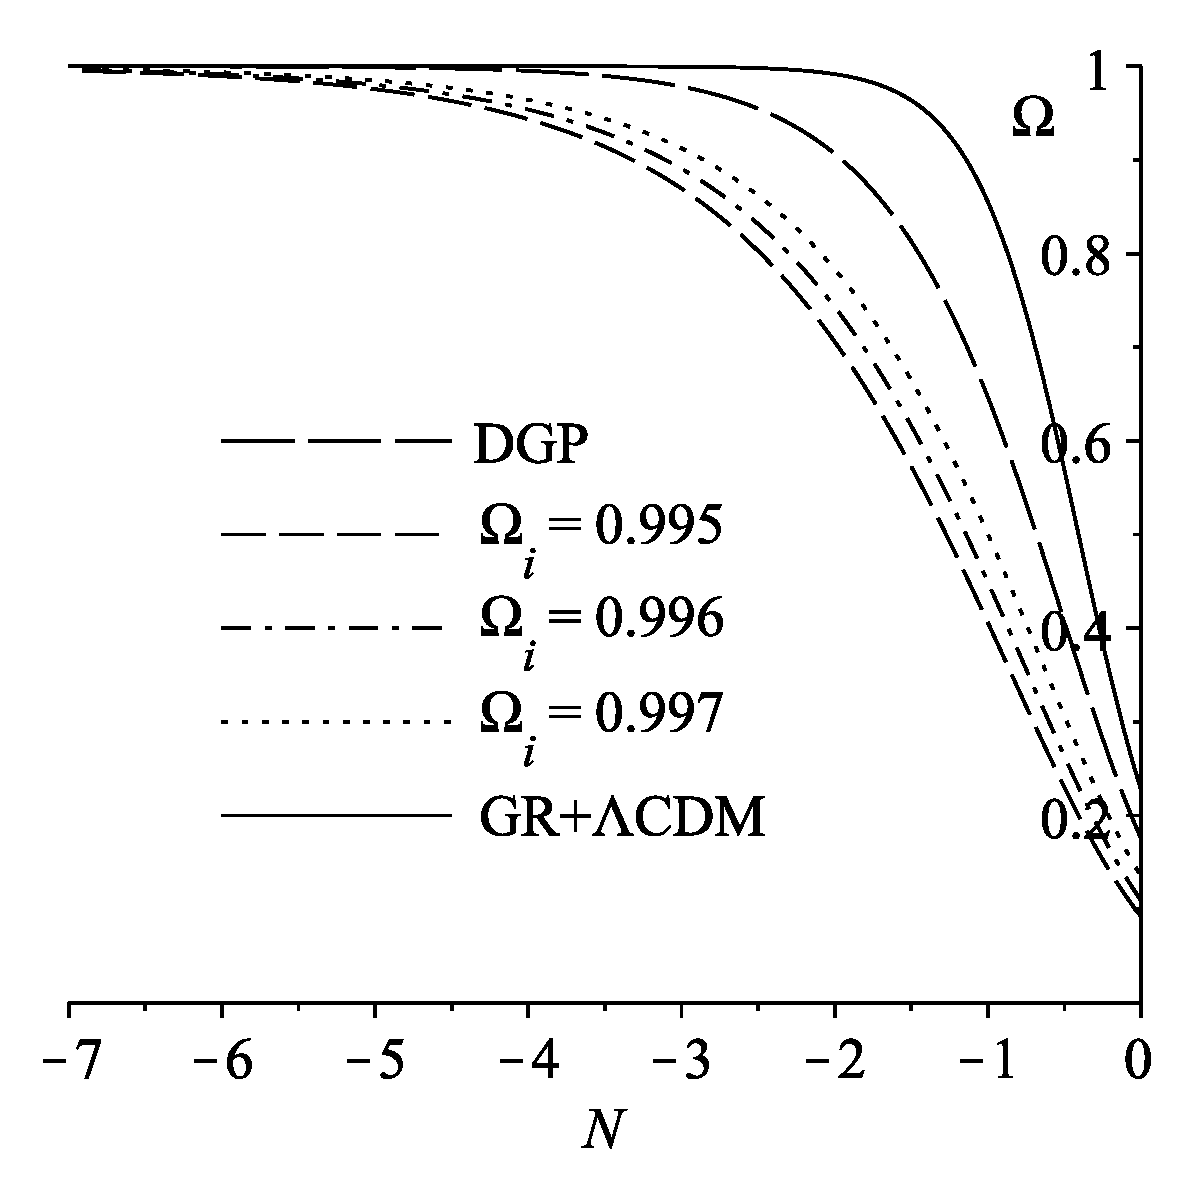
\includegraphics[width=0.49\columnwidth]{figures/dgpomegas.eps}
% For long captions include a short version for the List of Figures/Tables sections in square brackets as below.
\caption[Evolutions of $\delta$ and $\Omega$ for DGP]{Evolution of the density perturbation (left) and the density parameters (right) for the matched DGP/IDE models, each with a different $\Omega_i$,
and a GR+$\Lambda$CDM model.
\label{fig:matched}}
\end{figure}

Vector is better (EPS or PDF) if you can manage it. If you are exporting graphs from Microsoft Excel for example, place the chart in its own sheet and print it to PDF. Then, using Acrobat or similar, crop the whitespace off the PDF. This is the most reliable way I have found to include vector graphics from Microsoft Office.